% =====================================
% CAPÍTULO 3: METODOLOGÍA
% =====================================

\section{Metodología}

La metodología desarrollada en este trabajo tiene como objetivo implementar y validar el
ensayo Fiber-Bundle Pull-Out (FBPO) como técnica de caracterización interfacial a mesoescala
en materiales compuestos reforzados con fibras. Dado que el FBPO no corresponde a un
ensayo completamente estandarizado, la metodología se concibe como una adaptación
experimental controlada, orientada a asegurar reproducibilidad, trazabilidad y coherencia
en la determinación de la resistencia al corte interfacial.

El enfoque adoptado es de carácter experimental y se estructura en una secuencia de etapas
que abarcan el diseño y fabricación del sistema de ensayo, la preparación de probetas,
la ejecución de los ensayos FBPO y el procesamiento estadístico de los resultados. La unidad
de estudio considerada es una hebra completa de fibra de carbono, lo que sitúa el análisis en
una escala intermedia entre los ensayos micromecánicos de filamento único y los ensayos
macroscópicos de laminados.

Los valores de resistencia al corte interfacial reportados corresponden a una medida
aparente de la IFSS, dependiente del modelo de reducción empleado y de las condiciones
geométricas y de ensayo. En consecuencia, la metodología enfatiza el control de variables
críticas tales como la alineación axial, la longitud embebida, la velocidad de ensayo y el
criterio de muestra válida, así como el uso de prácticas de trazabilidad inspiradas en normas
ISO y DIN afines.

El diseño metodológico se organiza en seis etapas principales, que permiten abordar de
manera sistemática la implementación del ensayo FBPO y el análisis comparativo de la
adhesión fibra–matriz entre los sistemas evaluados.

\subsection{Materiales}

\subsubsection{Fibras de carbono utilizadas}

Para la fabricación de las probetas FBPO se emplearon dos tipos de tejido de fibra de carbono
provenientes del mismo proveedor, ambos con un gramaje nominal de 245~g/m\textsuperscript{2}, un
ancho de 100~cm y un ligamento Köper~2/2 (Twill~2/2). La utilización de tejidos con arquitectura
equivalente permite asegurar condiciones geométricas comparables en la extracción de hebras,
de modo que las diferencias observadas en el comportamiento interfacial puedan atribuirse
principalmente a características intrínsecas de la fibra.

Si bien ambos materiales comparten la misma arquitectura textil, cada uno corresponde a un
sistema de fibras distinto en términos de su masa lineal y, potencialmente, de su tratamiento
superficial (\textit{sizing}), lo que permite evaluar su influencia sobre la adhesión fibra–matriz
bajo condiciones experimentales controladas. En el ensayo FBPO, la unidad de estudio corresponde
a una hebra completa extraída del tejido, por lo que el tejido actúa únicamente como material de
origen para la obtención de las hebras ensayadas.

El primer material corresponde a un tejido basado en fibras \textbf{Tenax\textsuperscript{\textregistered}-E
HTA40 / 3k / HT} (ECC-Style~462), certificado para aplicaciones aeronáuticas. Este sistema presenta
filamentos de alta tenacidad y un \textit{sizing} compatible con resinas epóxicas de grado estructural,
lo que sugiere una buena humectación y estabilidad de la interfaz fibra–matriz. La etiqueta técnica
del fabricante se muestra en la Fig.~\ref{fig:fibraA_label}.

ETIQUETA

El segundo material corresponde a un tejido de fibra de carbono \textbf{HT 3k / 200~tex}, también en
ligamento Köper~2/2. Si bien comparte geometría y número de filamentos por hebra con la fibra Tenax,
posee una masa lineal distinta y un \textit{sizing} no especificado para aplicaciones aeronáuticas,
lo que potencialmente puede modificar la energía superficial y la fricción post–despegue en el
ensayo FBPO. Su correspondiente etiqueta se muestra en la Fig.~\ref{fig:fibraB_label}.

ETIQUETA

Ambos materiales fueron manipulados siguiendo prácticas de trazabilidad consistentes con DIN~29965
(registro de lote, masa lineal y especificaciones nominales). Las hebras fueron separadas del tejido
mediante el mismo procedimiento de extracción manual, con el objetivo de evitar daño superficial
o contaminación, manteniendo la coherencia entre series de fabricación. Esta selección de materiales
permite aislar el efecto del \textit{sizing} y comparar la adhesión fibra–matriz bajo condiciones
experimentales controladas.

\subsection{Diseño general de la investigación}

El diseño experimental se estructuró para cumplir los objetivos planteados mediante la
implementación controlada de un ensayo reproducible a mesoescala, considerando una hebra
de fibra de carbono como unidad de estudio. El estudio corresponde a un diseño experimental
comparativo de un factor principal, en el cual se evaluó la influencia del tipo de fibra
—y, en particular, de su tratamiento superficial o \textit{sizing}— sobre la interacción
interfacial fibra–matriz.

Se utilizaron hebras provenientes de dos proveedores distintos, correspondientes a un mismo
tipo nominal de fibra, de modo de aislar el efecto del recubrimiento superficial bajo
condiciones experimentales equivalentes. La comparación entre ambos sistemas de fibra
constituyó el caso de estudio central de la investigación. El alcance metodológico se
limitó a la fase experimental y al análisis estadístico de los resultados, sin considerar
modelación numérica ni efectos de degradación ambiental.

Para asegurar la validez interna del estudio, se controlaron variables críticas de ejecución
—alineación axial, longitud embebida, velocidad de ensayo y criterio de muestra válida— y se
documentó el estado del material, incluyendo la condición de la hebra y la ruta de curado de
la resina. Las probetas se asignaron de manera balanceada a las cavidades del molde y las
condiciones de ensayo se mantuvieron constantes dentro de cada campaña experimental. El
tamaño muestral por proveedor se definió en función de la variabilidad observada y de la
necesidad de realizar contrastes estadísticos con potencia suficiente, manteniendo un
registro explícito de exclusiones y sus causas.

En concordancia con \cite{DeLeon2022}, se adoptó una arquitectura de moldeo horizontal con
\emph{multicavidades} y dispositivos de alineación geométrica para controlar la longitud de
embebido y minimizar la dispersión asociada a desalineaciones. Las prácticas de sujeción y
alineación se inspiraron en \textbf{ISO 19375} y \textbf{DIN SPEC 19289} (para
\textit{single-fibre pull-out}), mientras que \textbf{ISO 3341} orientó el acondicionamiento
y la manipulación de hebras; \textbf{DIN 29965} respaldó la trazabilidad y especificación del
hilo de carbono utilizado \cite{ISO19375,DINSPEC19289,ISO3341,DIN29965}.

Finalmente, se definió un esquema de reporte mínimo que incluyó la identificación de
materiales y lotes, parámetros de fabricación y ensayo, criterios de validez, estadísticos
descriptivos por grupo y la métrica de IFSS aparente con su incertidumbre asociada. Este
marco metodológico guía la implementación detallada por etapas y asegura que las conclusiones
deriven de diferencias reales de material y proceso, y no de artefactos de montaje o de
reducción de datos.

\subsection{Etapas de desarrollo}

\subsubsection{Etapa 1: Revisión de antecedentes bibliográficos}

En una primera etapa se realizó una revisión sistemática de la literatura orientada a la
caracterización interfacial mediante ensayos de tracción y adhesión a nivel micro y mesoescala,
incluyendo métodos como el \textit{Single-Fiber Pull-Out}, \textit{Microdroplet}, \textit{Iosipescu}
y el \textit{Fiber-Bundle Pull-Out}. El objetivo de esta revisión fue identificar criterios
metodológicos relevantes para la implementación del ensayo FBPO a mesoescala, en particular
parámetros geométricos, condiciones de embebido y estrategias de sujeción que permitieran
asegurar comparabilidad con estudios previos.

Asimismo, se analizaron las directrices de normas internacionales afines, tales como
\textbf{DIN SPEC 19289}, \textbf{ISO 3341} y \textbf{DIN 29965}, las cuales aportan lineamientos
sobre control dimensional, alineación axial, acondicionamiento de hebras y trazabilidad del
material de refuerzo. A partir de esta revisión se incorporaron recomendaciones relativas al
reporte explícito de la \emph{IFSS aparente} y de su modelo de reducción, al control de variables
críticas de ejecución (velocidad de ensayo, longitud embebida $\ell_e$, alineación y criterio
de muestra válida), y al contraste de tendencias mediante métricas complementarias
\cite{Fischer2020,Liu2021,AhmadvashAghbash2024IMR}.

De forma complementaria, se definió una estrategia de búsqueda reproducible, que consideró
bases de datos especializadas, palabras clave y filtros por año y tipo de documento, junto
con una plantilla de extracción de datos. Dicha plantilla permitió sistematizar, para cada
estudio analizado, el sistema fibra–resina y su \textit{sizing}, la longitud embebida objetivo
y su método de medición, la velocidad de ensayo, el esquema de sujeción y alineación, el
criterio de muestra válida, la forma de identificación del despegue y el modelo de reducción
empleado.

Como resultado de esta etapa se obtuvo un compendio de rangos operativos recomendados
(p.\,ej., $\ell_e$ y sus tolerancias, velocidad de cruceta y acondicionamiento de hebras),
una lista de verificación para el control de variables experimentales y un esquema de
reporte mínimo que incluye la métrica de IFSS aparente, su incertidumbre asociada y los
criterios de validez del ensayo. Este insumo constituyó la base para parametrizar el diseño
experimental de las etapas posteriores, manteniendo coherencia y trazabilidad con la
literatura y las normas seleccionadas.

ANEXO (IFFS BIBLIOGRÁFICA)

\subsubsection{Etapa 2: Diseño del sistema experimental}

En la segunda etapa se desarrolló el diseño del sistema experimental mediante modelado asistido
por computadora en el software \textit{Autodesk Inventor}. Se elaboró el modelo tridimensional del
molde negativo para la fabricación de probetas de ensayo, considerando explícitamente las dimensiones
de embebido de la hebra y el control de la alineación axial durante el ensayo FBPO. Este diseño
constituyó la base para asegurar la precisión geométrica del ensayo y la reproducibilidad entre
probetas.

El molde negativo fue fabricado mediante impresión 3D en filamento de ácido poliláctico (PLA),
material seleccionado por su adecuada precisión dimensional, bajo costo y facilidad de
reproducción. Esta elección permitió obtener moldes reutilizables con geometría consistente,
facilitando la fabricación de múltiples probetas bajo condiciones controladas. En la
\Cref{fig:modelo_pla_negativo} se muestra el molde negativo impreso en PLA, el cual incorpora
una arquitectura \emph{multicavidad} con canales de sección constante y topes geométricos que
definen de manera reproducible la longitud de embebido $\ell_e$, en concordancia con la estrategia
propuesta por \cite{DeLeon2022}.

Como criterio de diseño, se priorizó que los canales del molde mantuvieran una sección constante
a lo largo de toda su longitud y que los topes geométricos fijaran $\ell_e$ sin requerir ajustes
posteriores, favoreciendo la repetibilidad entre cavidades y reduciendo la dispersión geométrica
entre probetas. El control de la alineación axial se integró directamente en el modelo CAD,
asegurando superficies de referencia planas y continuidad geométrica a lo largo del eje de la
hebra, de modo que el conjunto molde–probeta pudiera montarse de forma coaxial en la máquina de
tracción.

La \Cref{fig:modelo_pla_negativo} permite identificar estos elementos de diseño y visualizar su
disposición geométrica, evidenciando cómo el sistema experimental aborda de manera integrada el
control de la longitud embebida, la alineación axial y la repetibilidad del ensayo FBPO.

\begin{figure}[h!]
  \centering
  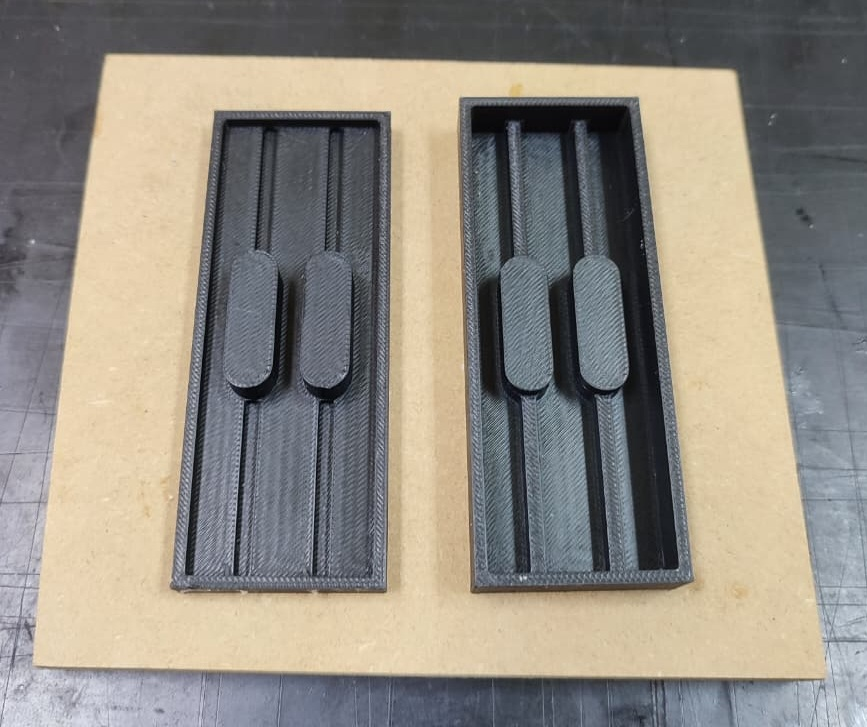
\includegraphics[width=0.5\textwidth]{Modelo_pla_negativo.jpeg}
  \captionsetup{justification=centering, singlelinecheck=false}
  \caption{Molde negativo impreso en PLA (multicavidad) con canales y topes geométricos para fijar \(\ell_e\).}
  \label{fig:modelo_pla_negativo}
\end{figure}

\subsubsection{Etapa 3: Fabricación de moldes de silicona}

En la tercera etapa se fabricaron moldes de silicona a partir de los modelos negativos impresos
en PLA, mediante el vertido de silicona líquida en las cavidades correspondientes. Una vez
curada, la silicona permitió obtener moldes blandos con la geometría requerida para el colado
de las probetas FBPO. Esta técnica fue seleccionada por su flexibilidad, estabilidad dimensional
y compatibilidad con resinas termoestables, lo que asegura la reproducción consistente de la
geometría definida en el molde rígido y facilita la fabricación seriada de probetas.

El material elastomérico empleado corresponde a una silicona RTV de dureza nominal
$\sim$~Shore~A~30, seleccionada específicamente para facilitar la liberación limpia de las
probetas y minimizar la probabilidad de daño local durante el desmoldeo. Esta elección
contribuye a reducir variaciones no deseadas en la longitud embebida $\ell_e$ y a preservar
la integridad geométrica de las cavidades a lo largo de múltiples ciclos de uso. La
\Cref{fig:silicona_caucho} muestra el sistema de silicona utilizado para la fabricación del
molde blando.

Durante esta etapa se priorizó la conservación de la geometría definida en el negativo de PLA
y la obtención de una superficie interna uniforme en las cavidades de silicona, de modo que el
colado posterior de la resina se realizara sin interferencias ni defectos superficiales. La
combinación de un molde rígido impreso en 3D y un molde blando de silicona RTV permitió integrar
control geométrico, facilidad de desmoldeo y repetibilidad, aspectos clave para la validez
experimental del ensayo FBPO.

\begin{figure}[h!]
  \centering
  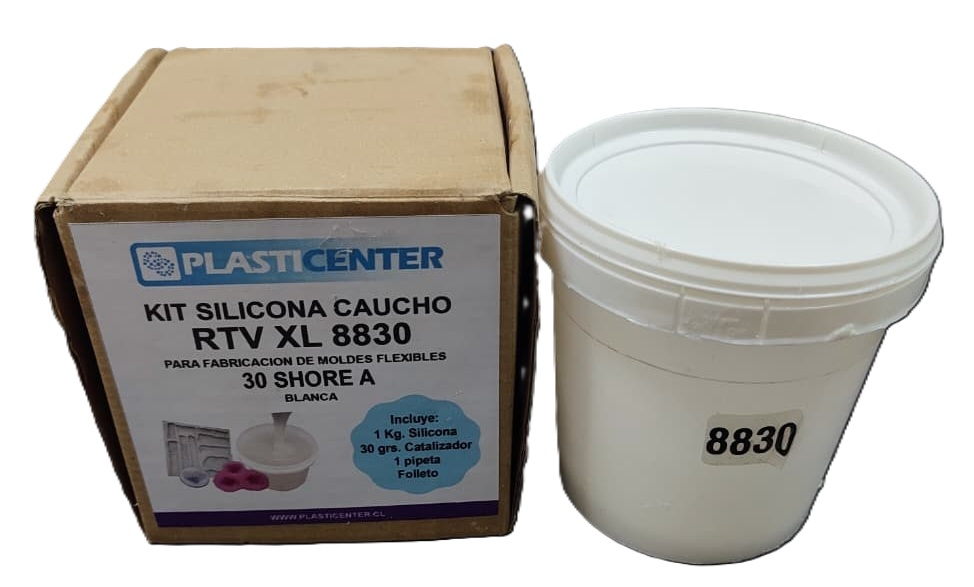
\includegraphics[width=0.5\textwidth]{Silicona_caucho.jpeg}
  \captionsetup{justification=centering, singlelinecheck=false}
  \caption{Sistema de silicona RTV empleado para la fabricación del molde blando (Shore A~30, kit silicona
  + catalizador).}
  \label{fig:silicona_caucho}
\end{figure}

\subsubsection{Etapa 4: Fabricación de probetas}

En la cuarta etapa se fabricaron las probetas de ensayo utilizando los moldes de silicona
desarrollados previamente. En cada cavidad se posicionó una hebra de fibra de carbono, la cual
fue embebida parcialmente en una resina epóxica líquida, de acuerdo con la longitud de embebido
$\ell_e$ definida por los topes geométricos del molde. Se emplearon hebras provenientes de dos
proveedores distintos, con el objetivo de comparar el efecto de posibles diferencias en el
recubrimiento superficial o \textit{sizing} sobre la resistencia interfacial.

Con el fin de asegurar que el área embebida correspondiera estrictamente a la geometría diseñada,
la porción no embebida de la hebra fue protegida mediante el recubrimiento con cinta de
politetrafluoroetileno (PTFE, teflón). Esta medida permitió evitar el avance no controlado de la
resina por capilaridad a lo largo de la hebra durante el colado y el curado, preservando así el
área embebida efectiva $A_e$ y reduciendo una fuente potencial de variabilidad experimental. El
correcto posicionamiento de la hebra, su tensión inicial y la integridad del recubrimiento de
teflón fueron verificados visualmente antes del colado de la resina.

Posteriormente, las probetas fueron sometidas a un proceso de curado y postcurado conforme a las
especificaciones del fabricante de la resina, asegurando una polimerización completa y estable
del sistema matriz. La secuencia de fabricación se resume en la \Cref{fig:etapas_probeta}, donde
se ilustran las etapas de: (a) cavidades de silicona, (b) posicionamiento y tensión inicial de la
hebra con protección en teflón, (c) colado y curado parcial, y (d) probeta desmoldeada. Este
registro visual respalda la trazabilidad cavidad–probeta y permite, cuando es pertinente, la
aplicación de un \emph{bloqueo por cavidad} en el análisis estadístico.

\begin{figure}[h!]
  \centering
  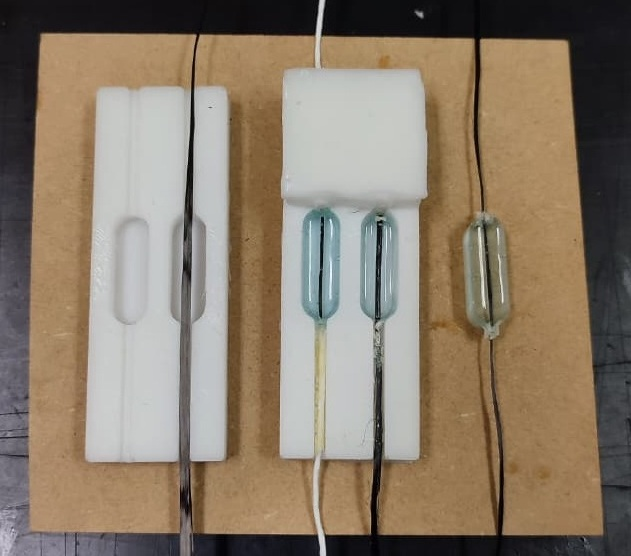
\includegraphics[width=0.5\textwidth]{Etapas_probeta.jpeg}
  \captionsetup{justification=centering, singlelinecheck=false}
  \caption{Secuencia de fabricación de probetas FBPO: cavidad de silicona, posicionamiento de hebra,
  colado/curado y desmoldeo.}
  \label{fig:etapas_probeta}
\end{figure}

Como criterio operativo, se mantuvo constante la longitud de embebido definida por los topes del
molde, se verificó el correcto asentamiento de la hebra en la cavidad antes del colado y se
respetaron los tiempos y temperaturas de curado indicados por el proveedor de la resina para todas
las probetas de una misma serie. Con el fin de preservar la comparabilidad entre ambos proveedores
de fibra, las probetas se fabricaron bajo las mismas condiciones de mezcla, vertido y curado, y se
etiquetaron de forma consistente (proveedor – lote – cavidad) para su trazabilidad durante el
procesamiento y análisis de los datos. La \Cref{fig:etapas_probeta} sirve además como guía visual
para reproducir el procedimiento con la misma secuencia y manipulación en diferentes lotes de
fabricación.

\subsubsection{Etapa 4.1: Caracterización mecánica de las resinas epóxicas}

Se emplearon sistemas epóxicos de baja viscosidad (resina + endurecedor) adecuados para el colado
en cavidades estrechas, con el objetivo de asegurar un buen mojado de la hebra y minimizar la
formación de burbujas. La \Cref{fig:resinas_epoxi} muestra los sistemas utilizados; la proporción
de mezcla y la cinética de curado se siguieron de acuerdo con las especificaciones del fabricante,
registrándose temperatura y tiempos con el fin de mantener consistencia entre lotes.

\begin{figure}[h!]
    \centering

    \begin{minipage}[b]{0.5\textwidth}
        \centering
        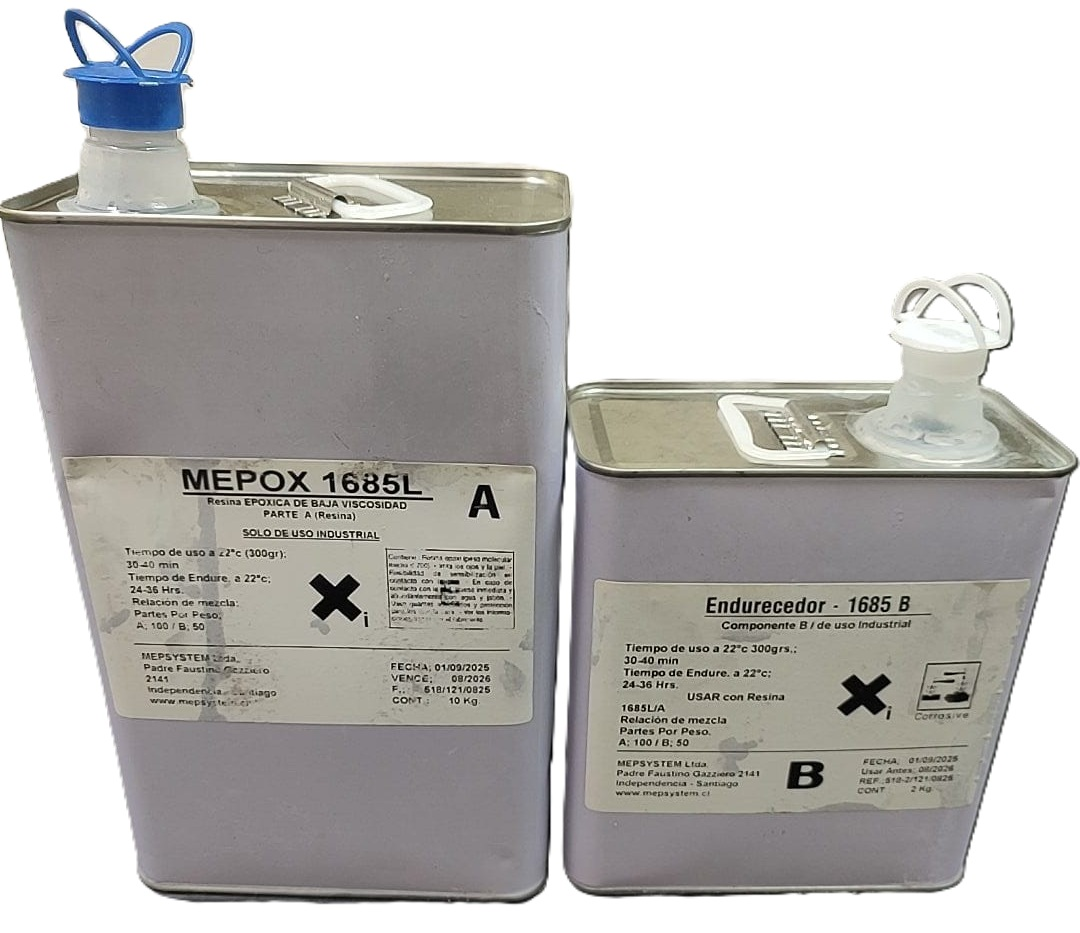
\includegraphics[height=6.3cm, keepaspectratio]{Resina_mepox_1685.jpeg}
    \end{minipage}%
    \begin{minipage}[b]{0.5\textwidth}
        \centering
        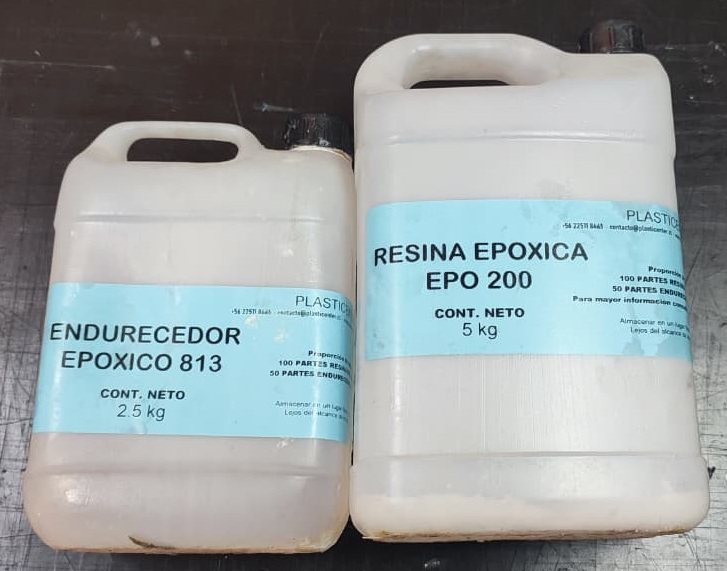
\includegraphics[height=6.3cm, keepaspectratio]{Resina_epo_200.jpeg}
    \end{minipage}

    \captionsetup{justification=centering, singlelinecheck=false}
    \caption{Sistemas epoxi de baja viscosidad utilizados. Izquierda: MEPOX 1685. Derecha: EPO 200.}
    \label{fig:resinas_epoxi}
\end{figure}

Con el propósito de disponer de parámetros mecánicos de referencia para la interpretación de los
resultados obtenidos mediante el ensayo FBPO, se realizó la caracterización en tracción de las
resinas empleadas en este estudio. Esta caracterización no tuvo por objetivo analizar en detalle
el comportamiento mecánico de las matrices, sino contextualizar las diferencias observadas en la
respuesta interfacial y descartar que estas se deban a variaciones significativas en las
propiedades intrínsecas de la resina.

Para ello se fabricaron probetas de resina pura utilizando geometría tipo IV, conforme a la norma
ASTM correspondiente para ensayos de tracción en polímeros termoestables. Todas las probetas fueron
ensayadas en una máquina de tracción universal Zwick Roell Proline Z05, registrándose las curvas
esfuerzo–deformación y la resistencia máxima a la tracción. El procedimiento de fabricación y
curado se mantuvo constante para ambas resinas, de modo que las diferencias observadas respondieran
exclusivamente a propiedades intrínsecas del sistema epoxi y no a variaciones de procesamiento.

\paragraph{Resina Mepox 1685L}
La primera formulación evaluada fue la resina epóxica Mepox 1685L, mezclada en la proporción
100A:50B indicada por el fabricante (componente A: Mepox 1685L; componente B: endurecedor 1685B).
Se confeccionaron diez probetas tipo IV bajo condiciones controladas de mezclado, vertido y curado.
Los ensayos de tracción permitieron obtener curvas esfuerzo–deformación consistentes, las cuales
fueron utilizadas como referencia para contextualizar el comportamiento de la matriz en los
ensayos FBPO.

\paragraph{Resina EPO 200}
La segunda formulación evaluada fue la resina epóxica EPO 200, mezclada con el endurecedor 813 en la
misma relación utilizada para el sistema Mepox. Dado que esta resina no cuenta con una ficha técnica
con propiedades mecánicas detalladas, su caracterización se realizó íntegramente mediante los
ensayos experimentales desarrollados en este trabajo. Se fabricaron probetas tipo IV siguiendo el
mismo procedimiento descrito anteriormente, registrándose curvas esfuerzo–deformación estables y
comparables entre sí. Los resultados obtenidos permitieron disponer de una referencia mecánica
mínima para la interpretación de los resultados FBPO y para analizar eventuales diferencias entre
sistemas matriz–fibra en términos de rigidez y resistencia en tracción.

\subsubsection{Etapa 5: Ejecución de los ensayos FBPO}

En la quinta etapa se ejecutaron los ensayos \textit{Fiber-Bundle Pull-Out} (FBPO) sobre las
probetas fabricadas, utilizando una máquina de tracción universal instrumentada y el montaje
experimental mostrado en la \Cref{fig:ensayo_fbpo}. Los ensayos se realizaron bajo condiciones
controladas de desplazamiento, registrándose de forma continua las curvas fuerza–desplazamiento
y documentándose los modos de falla observados en la interfaz fibra–matriz mediante registro
visual y fotográfico.

\begin{figure}[h!]
    \centering
    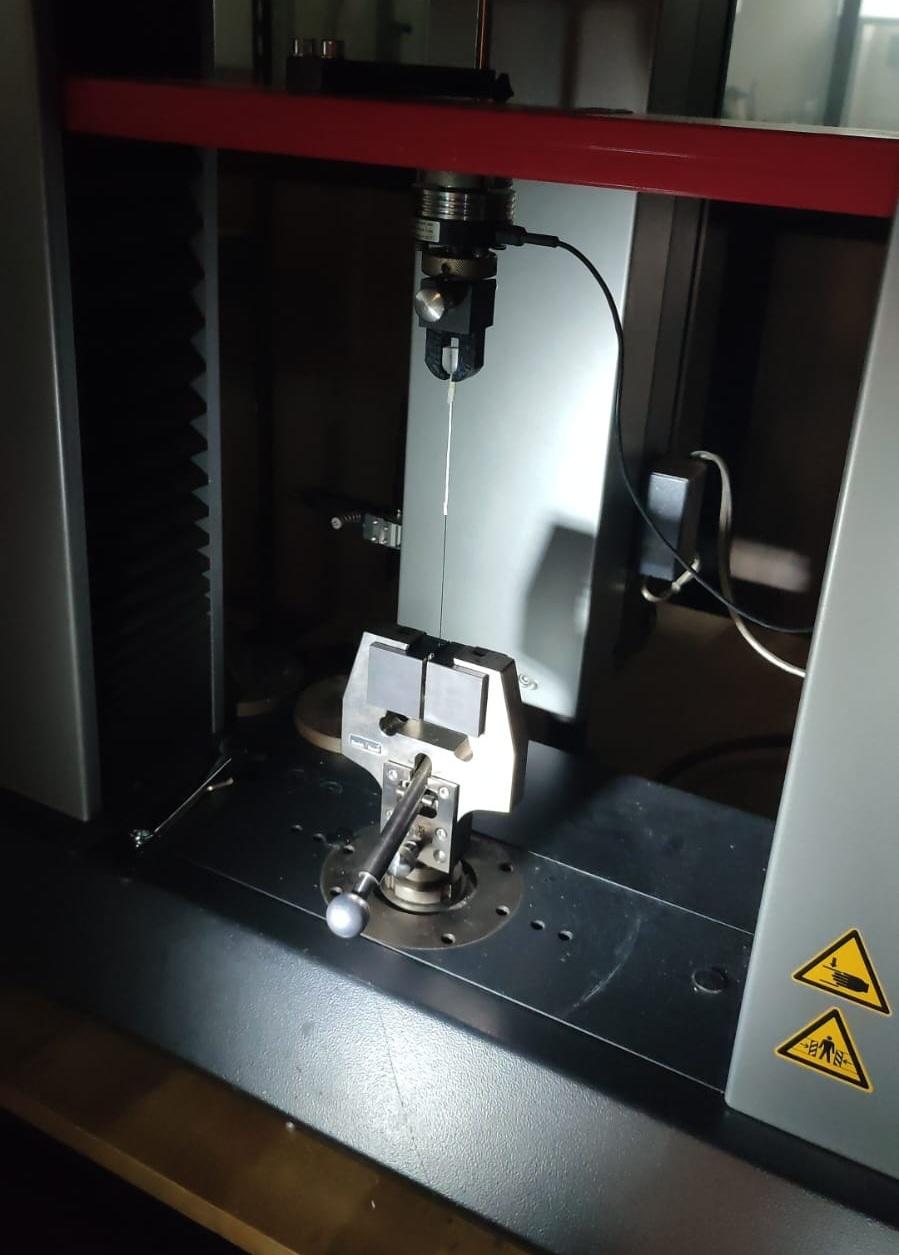
\includegraphics[height=7.5cm, keepaspectratio]{Ensayo_fbpo.jpeg}
    \captionsetup{justification=centering, singlelinecheck=false}
    \caption{Montaje experimental del ensayo \textit{Fiber-Bundle Pull-Out} (FBPO). }
    \label{fig:ensayo_fbpo}
\end{figure}

Previo a cada ensayo se realizó el \emph{zeroing} del sistema y se aplicó un \emph{preload}
mínimo, con el objetivo de asegurar el correcto asentamiento del conjunto probeta–mordazas y
eliminar holguras iniciales sin inducir daño interfacial. La velocidad de cruceta se mantuvo
constante para todas las probetas de una misma serie y se reportó junto con su tolerancia, de
modo de minimizar efectos asociados a la tasa de carga. La alineación axial del sistema se
verificó durante el montaje, asegurando que la carga se aplicara de manera coaxial a lo largo
del eje de la hebra.

Durante el ensayo se identificó explícitamente el punto de despegue interfacial \(P^{\ast}\),
asociado a la pérdida de adherencia entre la hebra y la matriz, a partir del cambio característico
en la pendiente de la curva fuerza–desplazamiento. Cuando correspondió, también se registró la
carga máxima alcanzada. La tasa de adquisición de datos se fijó a un valor suficiente para
resolver con claridad el evento de despegue y caracterizar el régimen posterior dominado por
fricción bajo la misma velocidad de cruceta.

Cada serie experimental incluyó un número suficiente de repeticiones para permitir el análisis
estadístico posterior. Se mantuvo invariable el procedimiento de montaje de las probetas en las
mordazas y la secuencia de preparación de la máquina a lo largo de toda la campaña experimental,
asegurando condiciones comparables entre grupos. El registro sistemático de las condiciones
nominales de cada corrida y de las observaciones visuales permitió mantener la trazabilidad
probeta–cavidad, requisito clave para el análisis estadístico y la interpretación de los valores
de IFSS aparente obtenidos.

\subsubsection{Etapa 6: Procesamiento y análisis de datos}

Los datos experimentales obtenidos se organizaron de acuerdo con el criterio de \emph{muestra válida},
asociando a cada registro su identificación completa (proveedor–lote–cavidad–fecha) y las variables
de ejecución relevantes (velocidad de ensayo y longitud embebida $\ell_e$ medida). Se realizó una
depuración básica de los datos, que incluyó la verificación de consistencia de unidades y la detección
de registros incompletos, junto con la elaboración de resúmenes descriptivos por grupo (medidas de
tendencia central y dispersión), manteniendo la trazabilidad explícita de cualquier exclusión.

La resistencia al corte interfacial se estimó en términos de una \textbf{IFSS aparente (FBPO)},
utilizando un modelo de reducción basado en la pendiente de la relación entre la carga de despegue
$P^{\ast}$ y el área embebida $A_e$, i.e., $\tau_{\text{IFSS,ap}} \approx \partial P^{\ast}/\partial A_e$,
obtenida mediante una regresión lineal forzada al origen. Para el cálculo del área embebida, las
hebras se aproximaron como cilindros de diámetro equivalente $d_{\text{eq}}$ y longitud embebida
$\ell_e$, de modo que $A_e = \pi d_{\text{eq}} \ell_e$. Para cada ajuste se reportaron la pendiente,
el coeficiente de determinación $R^2$ y los intervalos de confianza, junto con una revisión de
sensibilidad frente a puntos influyentes y, cuando correspondió, la aplicación de un esquema de
\emph{bloqueo por cavidad} para reducir el error residual \cite{Fischer2020,Liu2021,DeLeon2022}.

A partir de la métrica primaria $\tau_{\text{IFSS,ap}}$, calculada por probeta o por lote según el
caso, se realizaron contrastes estadísticos entre condiciones (proveedor A/B) mediante un ANOVA de
un factor. Previamente se verificaron los supuestos de normalidad y homogeneidad de varianzas; en
presencia de heterocedasticidad se utilizó la variante de Welch y, cuando fue pertinente, se
aplicaron comparaciones \emph{post hoc} (Tukey o Games–Howell). Los resultados se presentaron junto
con tamaños de efecto e incertidumbre asociada (intervalos de confianza y \emph{bootstrap} cuando
correspondió), enfatizando la identificación de tendencias robustas y su coherencia con antecedentes
reportados en la literatura.

Los valores de IFSS aparente obtenidos mediante FBPO se contrastaron además con antecedentes de
otros ensayos a mesoescala realizados en la misma institución (Iosipescu y tracción de hebras a
$45^\circ$ y $90^\circ$), con el objetivo de evaluar la aplicabilidad y confiabilidad del método.
En este contraste se priorizó la comparación de tendencias relativas entre sistemas fibra–matriz,
más que la intercambiabilidad numérica directa de los valores de IFSS, reconociendo el carácter
método-dependiente de la métrica obtenida \cite{Fischer2020,Liu2021,DeLeon2022}.

\subsection{Replicabilidad y validez}

El diseño experimental y los procedimientos se documentaron de manera que cualquier investigador
pueda reproducir las distintas etapas utilizando los mismos materiales, geometrías y parámetros
de ensayo. Se mantuvieron constantes las condiciones clave del experimento —alineación axial,
longitud embebida $\ell_e$ y velocidad de ensayo— y se registraron los insumos críticos, incluyendo
archivos CAD del molde, lotes de resina y fibra, fechas y condiciones ambientales de ensayo, junto
con evidencias del modo de falla observado.

Se definieron y aplicaron criterios explícitos de \emph{muestra válida}, así como causales de
descarte previamente establecidas, preservando en todo momento la trazabilidad cavidad–probeta.
Estas prácticas permitieron fortalecer la validez interna del estudio y reducir la influencia de
artefactos asociados al montaje, a la fabricación de probetas o al procesamiento de datos.

El uso de herramientas experimentales accesibles —modelado CAD, impresión 3D y ensayos de tracción
instrumentados— junto con un plan estadístico coherente, basado en ANOVA o su variante de Welch,
comparaciones \emph{post hoc} y reporte explícito de incertidumbre, refuerza la robustez de las
conclusiones y su comparabilidad interlote e interlaboratorio. En este marco, el ensayo
Fiber-Bundle Pull-Out se consolida como una técnica reproducible para el estudio de la adhesión
fibra–matriz a mesoescala.
